% This work is licensed under the Creative Commons
% Attribution-NonCommercial-ShareAlike 4.0 International License. To view a copy
% of this license, visit http://creativecommons.org/licenses/by-nc-sa/4.0/ or
% send a letter to Creative Commons, PO Box 1866, Mountain View, CA 94042, USA.

% (c) Eric Kunze, 2019

%%%%%%%%%%%%%%%%%%%%%%%%%%%%%%%%%%%%%%%%%%%%%%%%%%%%%%%%%%%%%%%%%%%%%%%%%%%%%%%
% Template for lecture notes and exercises at TU Dresden.
%%%%%%%%%%%%%%%%%%%%%%%%%%%%%%%%%%%%%%%%%%%%%%%%%%%%%%%%%%%%%%%%%%%%%%%%%%%%%%%

\documentclass[ %
ngerman, %
a4paper, %
sectionreset, %
chapterstyle=framed, %
sectionstyle=dotted, %
titlefont=osfamily %
]{../../../../texmf/tex/latex/mathscriptMathTUD/mathscriptMathTUD}

\usepackage[order=firstname, fractionappearence=lowerraise]{../../../../texmf/tex/latex/mathworkMathTUD/mathworkMathTUD}
%\usepackage[presentExercise]{../../texmf/tex/latex/exercisesMathTUD/exercisesMathTUD}

%%%%%%%%%%%%%%%%%%%%%%%%%%%%%%%%%%%%%%%%%%%%%%%%%%%%%%%%%%%%%%%%%%%%%%%%%%%%%%%

%---------------------------------------
% additional packages
%---------------------------------------

% none


%---------------------------------------
% general settings
%---------------------------------------

\name{Eric Kunze \& Lars Ortscheidt}
\matnr{Nummer}
\email{\href{mailto:eric.kunze@mailbox.tu-dresden.de}{\ttfamily eric.kunze@mailbox.tu-dresden.de}}

\modul{Numerische Mathematik}
\period{Sommersemester 2019}

%\tutor{Dr. Legrand}
%\group{Tag x. DS, (un)gerade Woche}

\lecturer{Prof. Dr. Andreas Fischer}
\faculty{Mathematik}
\institute{Numerik}
\professorship{Optimierung}

%%%%%%%%%%%%%%%%%%%%%%%%%%%%%%%%%%%%%%%%%%%%%%%%%%%%%%%%%%%%%%%%%%%%%%%%%%%%%%%
% specific commands

\lstset{language=Matlab,
	basicstyle=\ttfamily,
	keywordstyle=\bfseries,
	%commentstyle=
	%morecomment=[l]{!\ },% Comment only with space after !
	%stringstyle=\color{darkgray}\ttfamily,
	%backgroundcolor=\color{white},
	showstringspaces=false,
	numbers=left,
	numbersep=10pt,
	%numberstyle=\color{gray}\ttfamily,
	%identifierstyle=\color{black},
	xleftmargin=.1\textwidth, 
	xrightmargin=.1\textwidth,
	breaklines=true,
	frame=single,
	literate=%
	{Ö}{{\"O}}1
	{Ä}{{\"A}}1
	{Ü}{{\"U}}1
	{ß}{{\ss}}2
	{ü}{{\"u}}1
	{ä}{{\"a}}1
	{ö}{{\"o}}1
}

%%%%%%%%%%%%%%%%%%%%%%%%%%%%%%%%%%%%%%%%%%%%%%%%%%%%%%%%%%%%%%%%%%%%%%%%%%%%%%%


\begin{document}
    
    \chapter*{Praktische Umsetzung des SOR-Verfahrens}
    \begin{center}
    	\textit{Praktische Aufgabe P1 im Modul Math-Ba-NUM} \\
    	\Large{\bfseries \textsc{Lars Ortscheidt \& Eric Kunze}}
    \end{center}
    
    \section{Darstellung der Besetzung}
    Die Darstellung der Besetzung der jeweiligen Matrizen ist \cref{abb: besetzung}
	zu entnehmen.
	\begin{center}
		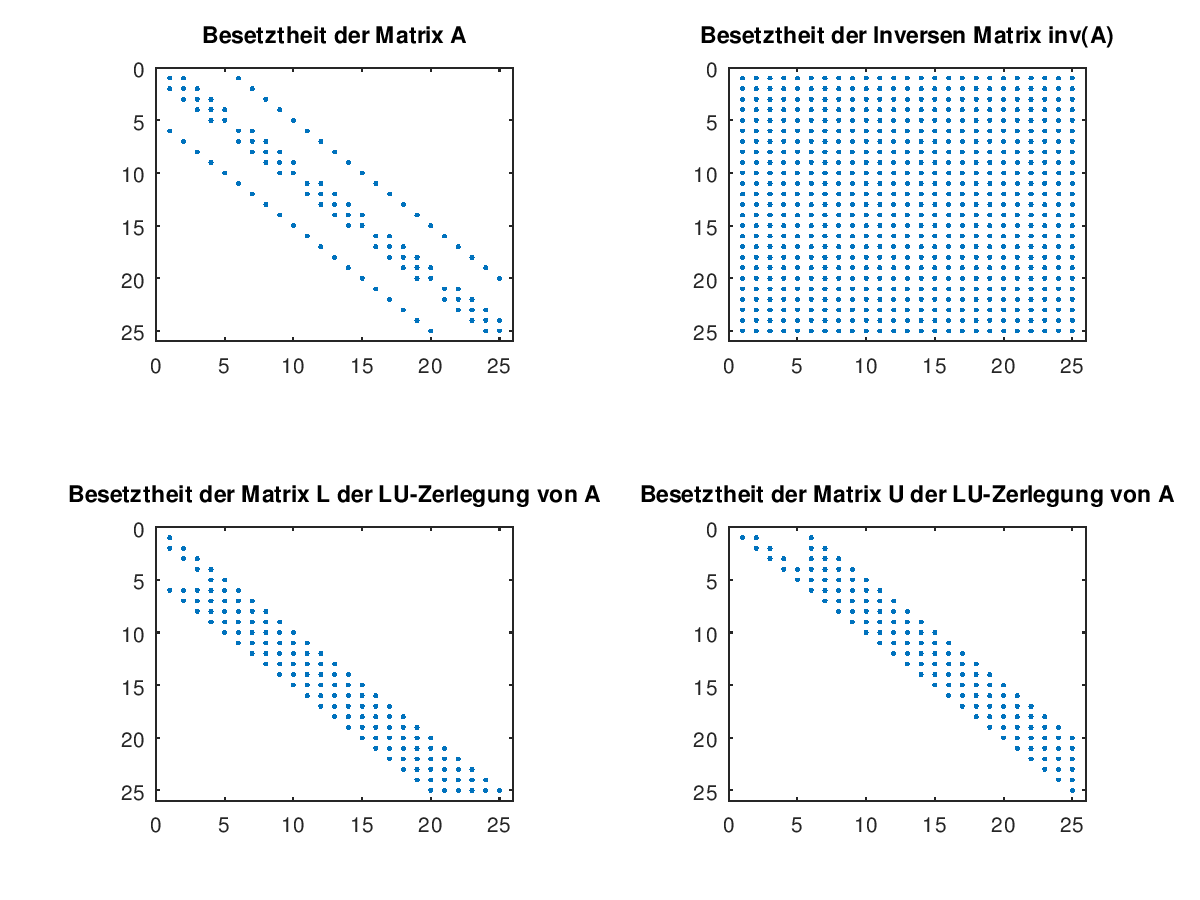
\includegraphics[scale=0.5]{besetztheit.png}
		\captionof{figure}{Besetzung der einzelnen Matrizen}
		\label{abb: besetzung}
	\end{center}
	
	Anhand der Darstellung ist erkennbar, dass die Eigenschaft der Dünnbesetztheit nicht invariant unter Inversion ist, d.h. die Inverse einer dünnbesetzten Matrix kann wie hier durchaus (nahezu) voll besetzt sein. Damit beeinflussen Inversionen auch die Geschwindigkeit eines Iterationsverfahrens negativ.
	
	Die LU-Zerlegung der Matrix $A$ existiert stets, da alle Matrizen $A$ unabhängig von ihrer Dimension immer regulär, symmetrisch und positiv definit sind.
	
	\section{Iterationsverfahren}
	Wir beschreiben hier kurz unsere Lösungsstrategie im SOR-Verfahren, welches im File \texttt{SOR.m} zu finden ist. Zu lösen sei das Gleichungssystem $Ax = b$. 
	
	Die erste Idee war die Implementierung mittels der Iterationsvorschrift $Mx = c$, wobei 
	\begin{equation*}
		M \defeq \left( L + \frac{1}{\omega} D \right)^{-1} \left( \frac{1 - \omega}{\omega} D - R \right) \quad \und \quad c \defeq \left( L + \frac{1}{\omega} D \right)^{-1} * b
	\end{equation*}
	Jedoch ist insbesondere die notwendige Inversion stets negativ auffallend, da aus den dünn besetzten Matrizen dann wieder (nahezu) vollbesetzte Matrizen entstehen.
	
	Aus diesem Grund verwenden wir im Folgenden die Darstellung ohne Inversion und damit die Iterationsvorschrift
	\begin{equation*}
		x^{k+1} \defeq x^k - \left( L + \frac{1}{\omega}D \right)^{-1} (Ax^k - b)
	\end{equation*}
	Dabei kann die Inversion in der konkreten Implementierung durch den Operator \texttt{$\backslash$} ersetzt werden, sodass also die eigentliche Iteration mit $B = L + \frac{1}{\omega} * D$ sich durch
\begin{lstlisting}[language=matlab, ]
while(n<=nmax && fehler>=tol)
	X      = X - B \ (A*X-b); % Iterationsschritt
	n      = n + 1;           % Iterationszaehler
	fehler = norm(A * X - b) / norm(b);
endwhile
\end{lstlisting}

	
    \section{Poisson-Gleichung}
    Wir betrachten die Lösung $u(x,y) = x^2 (1-x) y (1-y)$  der Poisson-Gleichung $- \Delta u(x,y) = g(x,y)$. Dann ist die Funktion $g$ durch 
    \begin{equation*}
    	g(x,y) = -\div \grad \left( x^2 (1-x) y (1-y) \right) = 2 \left( -x^2 + x^3 - (-1 + y) y + 3 x (-1 + y) y \right)
    \end{equation*}
    bestimmt. Dies ist im Programm die Funktion \texttt{poisson}.
    
    \section{Dokumentation der Iterationszahlen}
    
    Sei
    \begin{equation*}
    	f(x,y) = \sin(\pi * x) * \sin(\pi * y)
    \end{equation*}
    und 
    \begin{equation*}
    	g(x,y) = 2 \left( -x^2 + x^3 - (-1 + y) y + 3 x (-1 + y) y \right)
    \end{equation*}
    Die Werte für den Relaxationsparameter $\omega \in \menge{1, 1.8, \omega^\ast}$ beziehen sich jeweils auf die Berechnung mit \texttt{SOR}, für das CG-Verfahren wurde die Funktion \texttt{pcg} verwendet.
    
    \medskip
    
    \begin{minipage}{\dimexpr0.5\linewidth-\fboxrule-\fboxsep}
   	\centering
    \begin{tabular}{|r||rrr|r|}
    	\hline
    	\diagbox[dir=NW]{$N$}{$\omega$} & $1$ & $1.8$ & $\omega^\ast$ & CG \\
    	\hline \hline
    	  5 &   49 &   66 &  17 & 1 \\
    	 10 &  168 &   69 &  32 & 1 \\
    	100 & 1500 & 1500 & 299 & 1 \\
    	200 & 1500 & 1500 & 595 & 1 \\
    	\hline
    \end{tabular}
	\captionof{table}{Iterationszahlen für $f$}
	\end{minipage}
    \begin{minipage}{\dimexpr0.5\linewidth-\fboxrule-\fboxsep}
    \centering
    \begin{tabular}{|r||rrr|r|}
    	\hline
    	\diagbox[dir=NW]{$N$}{$\omega$} & $1$ & $1.8$ & $\omega^\ast$ & CG \\
    	\hline \hline
    	  5 &   49 &   66 &  17 &  11 \\
    	 10 &  165 &   69 &  33 &  22 \\
    	100 & 1500 & 1500 & 300 & 221 \\
    	200 & 1500 & 1500 & 598 & 447 \\
    	\hline
    \end{tabular}
	\captionof{table}{Iterationszahlen für $g$}
	\end{minipage}

	Aus diesen Werten sind mehrere Eigenschaften ersichtlich. Offensichtlich konvergiert das CG-Verfahren schneller als das SOR-Verfahren, was aber auch so zu erwarten war. Insbesondere bei der Betrachtung der Funktion $g$ lässt sich aber erahnen, dass bei noch größeren $N > 200$ sich die Iterationszahlen des CG-Verfahrens und des SOR-Verfahrens mit $\omega^\ast$ weiter annähern. 
	
	Betrachten wir das SOR-Verfahren isoliert, so nimmt die Iterationszahl für die Folge der $\omega$ i.d.R. kontinuierlich ab. $\omega=1$ beschreibt ja bekanntermaßen das Gauß-Seidel-Verfahren. Dieses kommt ohne den Relaxationsparameter aus und erreicht damit schlechtere Konvergenzeigenschaften. Das $\omega^\ast$ beschreibt den optimalen Relaxationsparameter, was man auch zeigen kann. Allgemein kann folgende Darstellung gefunden werden
	\begin{equation*}
		\omega^\ast = \frac{2}{1 + \sqrt{1 - \rho(D^{-1}(L+R))}}
	\end{equation*} 
	Damit wird dann die schnellste Konvergenz erreicht, was beispielsweise auch dazu führt, dass die maximale Iterationszahl nur mit $\omega^\ast$ unterschritten wird (betrachte z.B. $f$ und $N = 200$).
	
	Vergleicht man nun beide Funktionen $f$ und $g$, so stellt man fest, dass $f$ im Allgemeinen relativ ähnliche Iterationszahlen im SOR-Verfahren liefert wie $g$. Ein deutlicher Unterschied ist dagegen bei der Verwendung des CG-Verfahrens zu erkennen, was für $f$ stets nach einer Iteration konvergiert, dagegen für $g$ mitunter fast so viele Iterationen benötigt wie das SOR-Verfahren mit $\omega^\ast$.
	
	Besonders ist anhand dieser Aufgabe zu erkennen, dass nicht alle Verfahren gleich schnell konvergieren und auch für verschiedene Parameter innerhalb der Verfahren sich unterschiedliche Konvergenzeigenschaften ergeben.
	
	\section{Fehlerdarstellung}
	\newlength{\halfpage}
	\setlength{\halfpage}{\dimexpr0.5\linewidth-\fboxrule-\fboxsep}
	
	Im Folgenden ist die grafische Darstellung der Fehler in Abhängigkeit der Iterationszahl zu finden. Der (relative) Fehler wurde mithilfe von
	\begin{equation*}
		\frac{\norm{A*x - b}}{\norm{b}}
	\end{equation*}
	berechnet. Dabei haben wir eine dem SOR-Verfahren gleiche Funktion \texttt{fehlervec} erstellt, die das SOR-Verfahren simuliert, aber lediglich ein Vektor zurückgibt, dessen $i$-ter Eintrag der Fehler im $i$-ten Iterationsschritt ist. 

	\begin{figure}
		\centering
		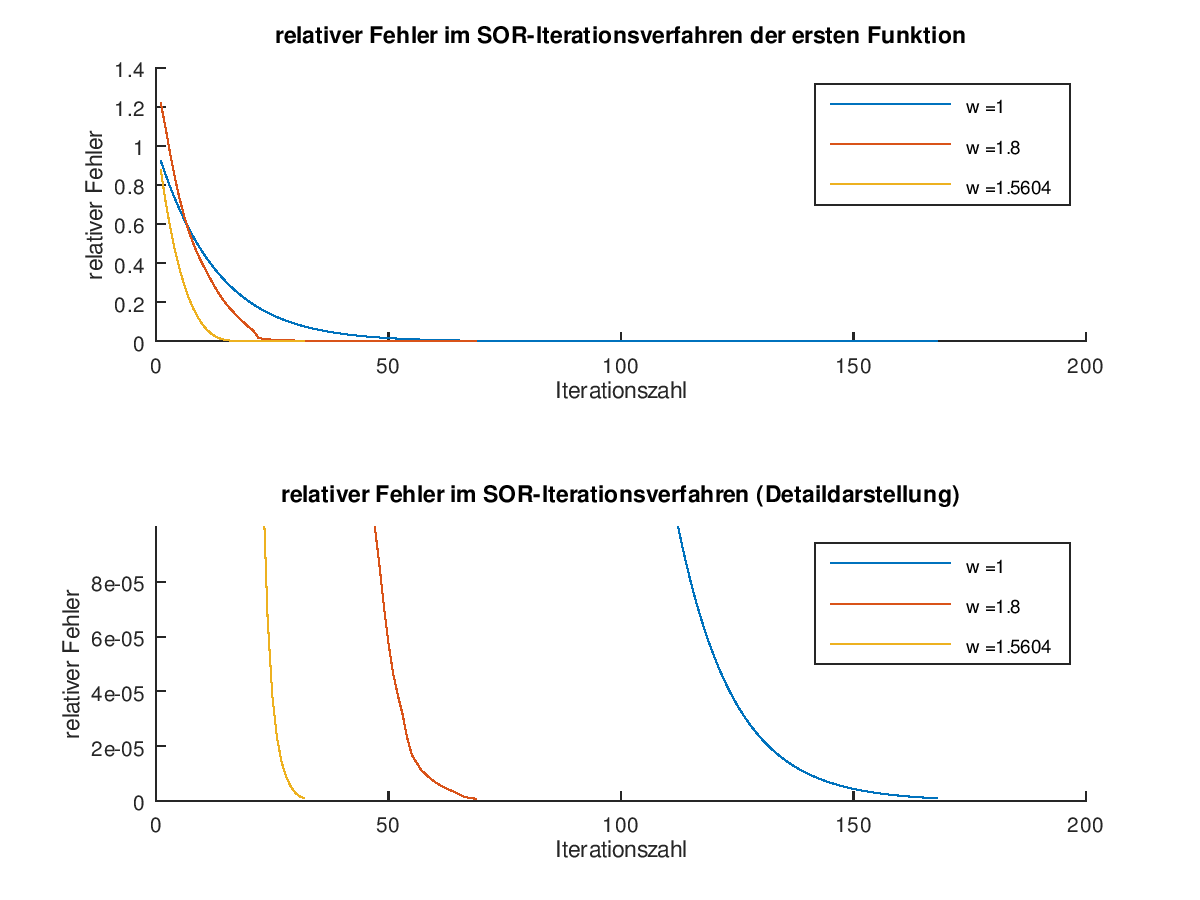
\includegraphics[width=0.75\linewidth]{fehlerplot1.png}
		\caption{Fehler in Abhängigkeit der Iteration von $f$}
		\bigskip \bigskip
		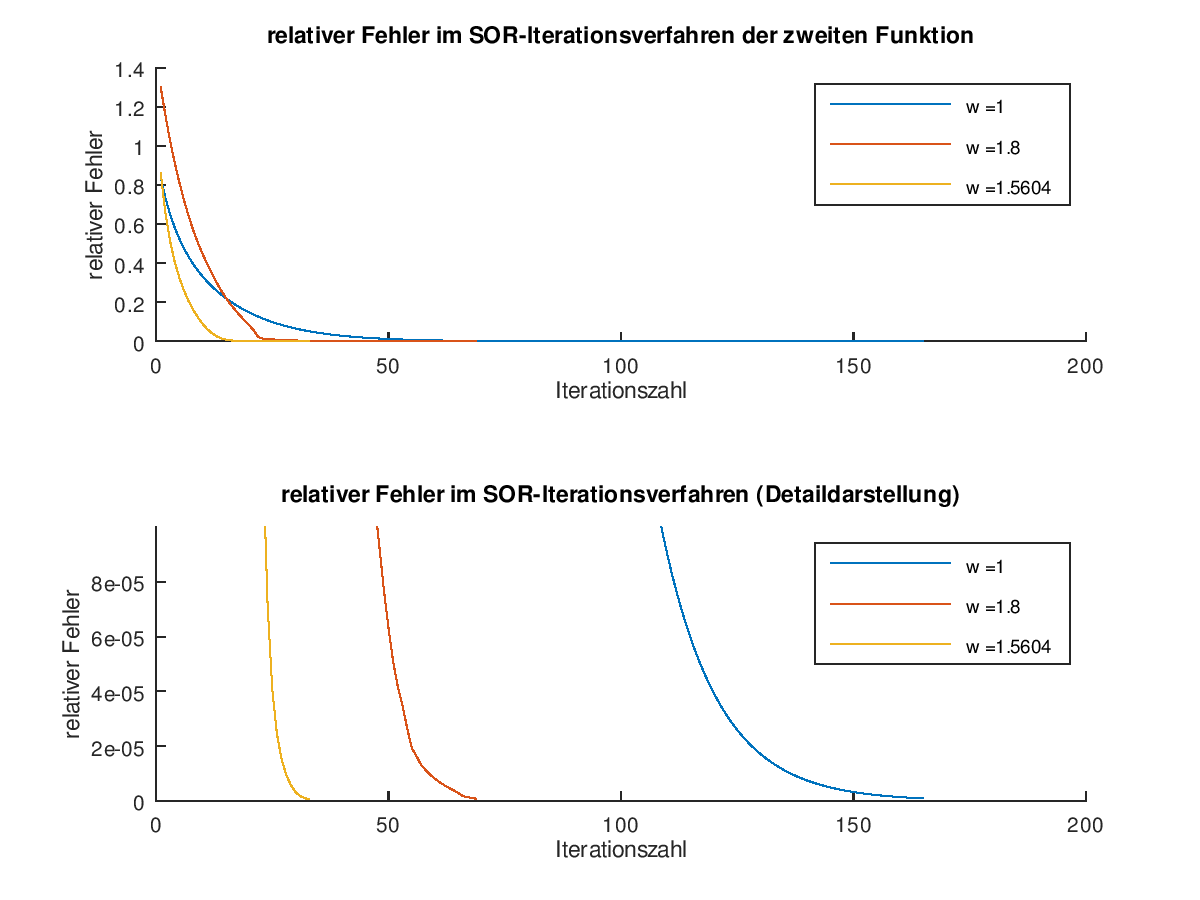
\includegraphics[width=0.75\linewidth]{fehlerplot2.png}
		\caption{Fehler in Abhängigkeit der Iteration von $g$}
	\end{figure}

	Es ist deutlich zu erkennen, dass die Konvergenz mit optimiertem $\omega^\ast$ schneller erreicht wird als im Gauß-Seidel-Verfahren oder mit $\omega = 1.8$. Zwischen den beiden Gleichungen $f$ und $g$ sind wie auch in den Iterationszahlen nur geringfügige Unterschiede zu erkennen.
\end{document}
